


\begin{frame}{Grid Cell Modeling \sof{1}{5}}



\twocol{0.6}{
\justifying

Grid Cells are {\bf neurons in the entorhinal cortex of mammals} that exhibit 
very specific patterns of activity that correlates strongly with the allocentric 
location of the animal.

\vspace{1em}
Virtually all existing computational models of grid cells are {\bf narrow 
models} that view grid cells as part of a specialized system for navigation.

\vspace{3em}
}{0.35}{
\vspace{-0.5em}
\begin{figure}
%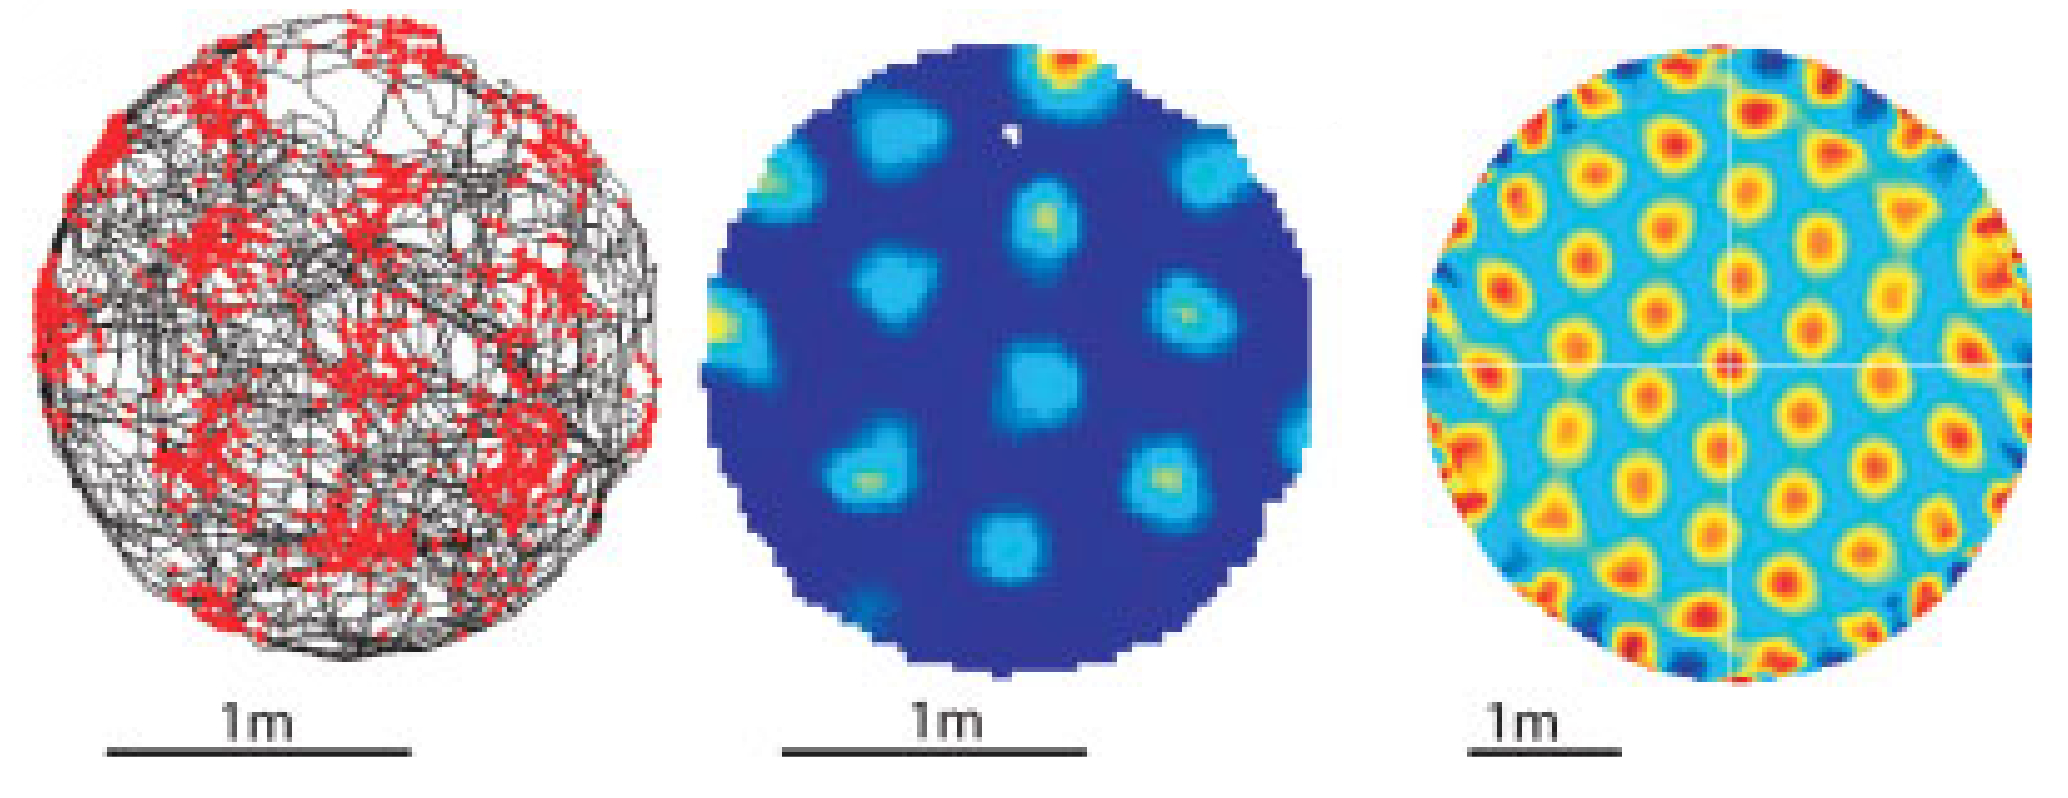
\includegraphics[width=\linewidth]{diss/gc_rate_auto.jpg}
\adjincludegraphics[width=\linewidth,valign=t]{diss/gc_rate_auto.jpg}

\vspace{-0.5em}
\caption{\scriptsize Typical visualization of the recorded activity of a grid 
cell~\cite{kerdels2015b}.}
\end{figure}
}


\twocol{0.25}{
\vspace{-1em}
\begin{figure}
%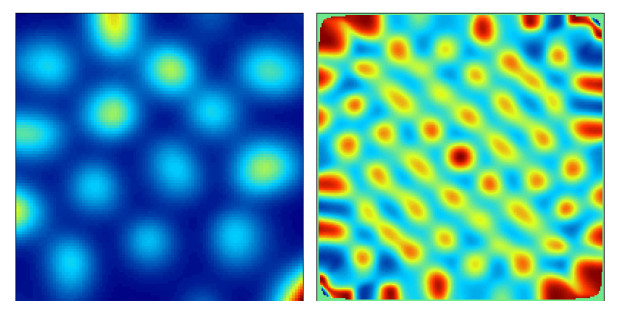
\includegraphics[width=\linewidth]{diss/gridsim.jpg}
\adjincludegraphics[width=\linewidth,valign=b]{diss/gridsim.jpg}

\vspace{-0.5em}
\caption{\scriptsize Activity pattern of a grid cell that was simulated by 
us~\cite{kerdels2015b}.}
\end{figure}

}{0.7}{
\justifying

We were the first to suggest that grid cell activity might reflect a {\bf 
general computational principle} that underlies not only the behavior of grid
cells but describes the behavior of (some) cortical cell groups in 
general~\cite{kerdels2013b,kerdels2015b}.

}

\begin{center}
\rule{2cm}{0.4pt}\\[0.5em]
\end{center}

\fc{kerdels2013b}{publications/2013-01/2013-01}\nombestpaper\\[1em]
\fc{kerdels2015b}{publications/2015-01/2015-01}

\end{frame}


\begin{frame}{Grid Cell Modeling \sof{2}{5}}

%\vspace{1em}
\justifying

\vspace{1.5em}
My dissertation~\cite{Kerdels2016} investigates {\bf entorhinal grid cells} in 
detail covering their neurobiological and functional 
properties~\cite{Kerdels2018b}, as well as existing computational models and 
their associated functional hypotheses.

\vspace{1.5em}
The main contribution of my work is the introduction of a {\bf new computational 
model} that views grid cell activity as expression of a {\bf general 
computational principle}. 

\twocol{0.52}{
\justifying

\vspace{0.5em}
At the core of this general principle lies the {\bf novel conjecture} that 
cortical neurons learn a representation of their {\bf entire} input space while 
competing locally with their peers.

\vspace{1.5em}
The dissertation was honoured with the \mbox{\bf faculty award} for the best 
scientific work in 2017. 
{\scriptsize [laudation:\vid{publications/2016-01/laudatio_fpreis_20171120.mp4}, 
presentation:\vid{publications/2016-01/fpreis_20171120.mp4}]}

}{0.4}{
\vspace{-0.5em}
\begin{figure}
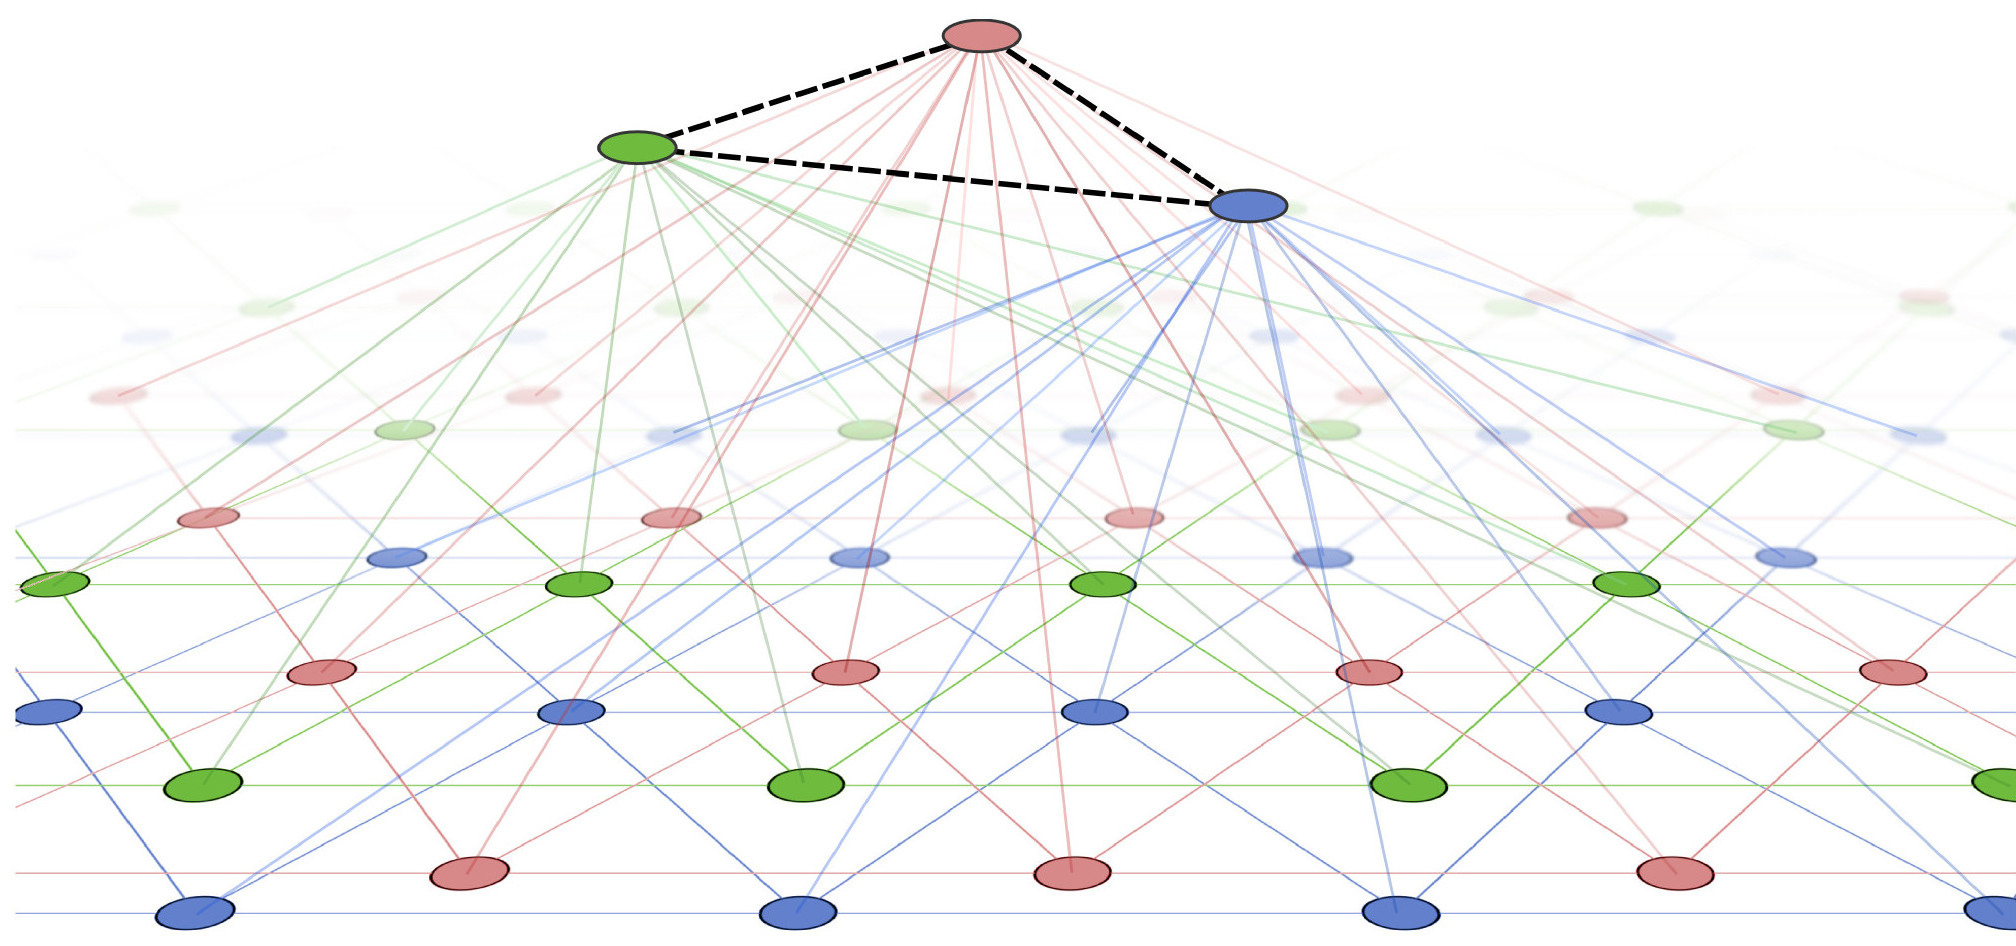
\includegraphics[width=\linewidth]{diss/rgng_ex.jpg}

\vspace{-1em}
\caption{\scriptsize Schematic view of a two-layer RGNG network used to 
simulate a group of grid cells~\cite{Kerdels2016}.}
\end{figure}

}

\vspace{0.5em}

\begin{center}
\rule{2cm}{0.4pt}\\[0.5em]
\end{center}

\fc{Kerdels2016}{publications/2016-01/2016-01}\\[1em]
\fc{Kerdels2018b}{publications/2018-02/2018-02}\\[1em]
\fcn{Kerdels2018c}{publications/2018-03/2018-03}\cover

\end{frame}



\begin{frame}{Grid Cell Modeling \sof{3}{5}}

%\vspace{1em}
\justifying

\vspace{1.5em}
Killian et al. discovered {\bf grid-like activity} of entorhinal cells that was 
not correlated with location but rather with the animal's {\bf gaze direction}.

\vspace{1.5em}
Since our model is based on a general computational principle and does not rely
on assumptions regarding navigation and orientation we were able to
{\bf model and replicate the observed 
phenomena}~\cite{Kerdels2016a,Kerdels2019}.


\vspace{0.5em}

\begin{figure}
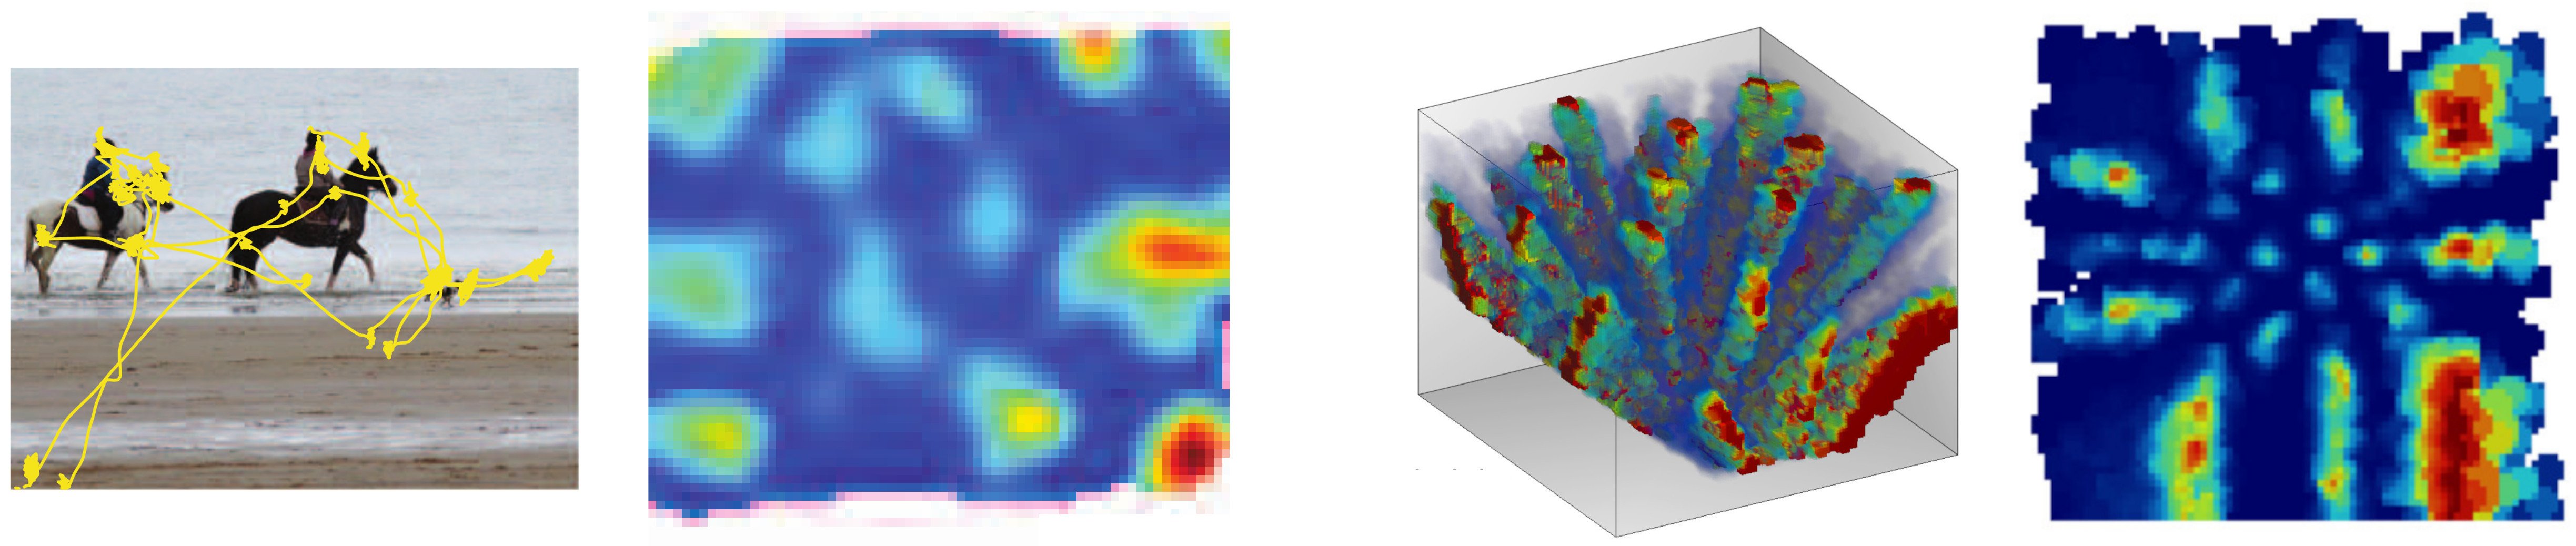
\includegraphics[width=0.9\linewidth]{diss/saccade_grids.jpg}

\vspace{-0.5em}
\caption{\justifying\scriptsize Grid-like activity that correlates with saccadic eye 
movements was observed in primates by Killian et al. (left). Modeling binocular
eye movements with our computational model results in a three-dimensional 
activation space that recreates the observed patterns when reduced to the 
two-dimensional viewing plane of the primate studied by Killian
(right)~\cite{Kerdels2016a,Kerdels2019}.}
\end{figure}

\vspace{-2em}

\begin{center}
\rule{2cm}{0.4pt}\\[0.5em]
\end{center}

\fc{Kerdels2016a}{publications/2016-03/2016-03}\bestpaper\\[1em]
\fc{Kerdels2019}{publications/2019-02/2019-02}

\end{frame}




\begin{frame}{Grid Cell Modeling \sof{4}{5}}

\vspace{1.5em}
\justifying
{\bf Noise Resilience} is a necessary property of neurobiological systems as 
they experience a wide range of interference factors and are built out of 
components that are non reliable in general.

\vspace{1em}

\twocol{0.4}{
\vspace{-2em}
\begin{figure}
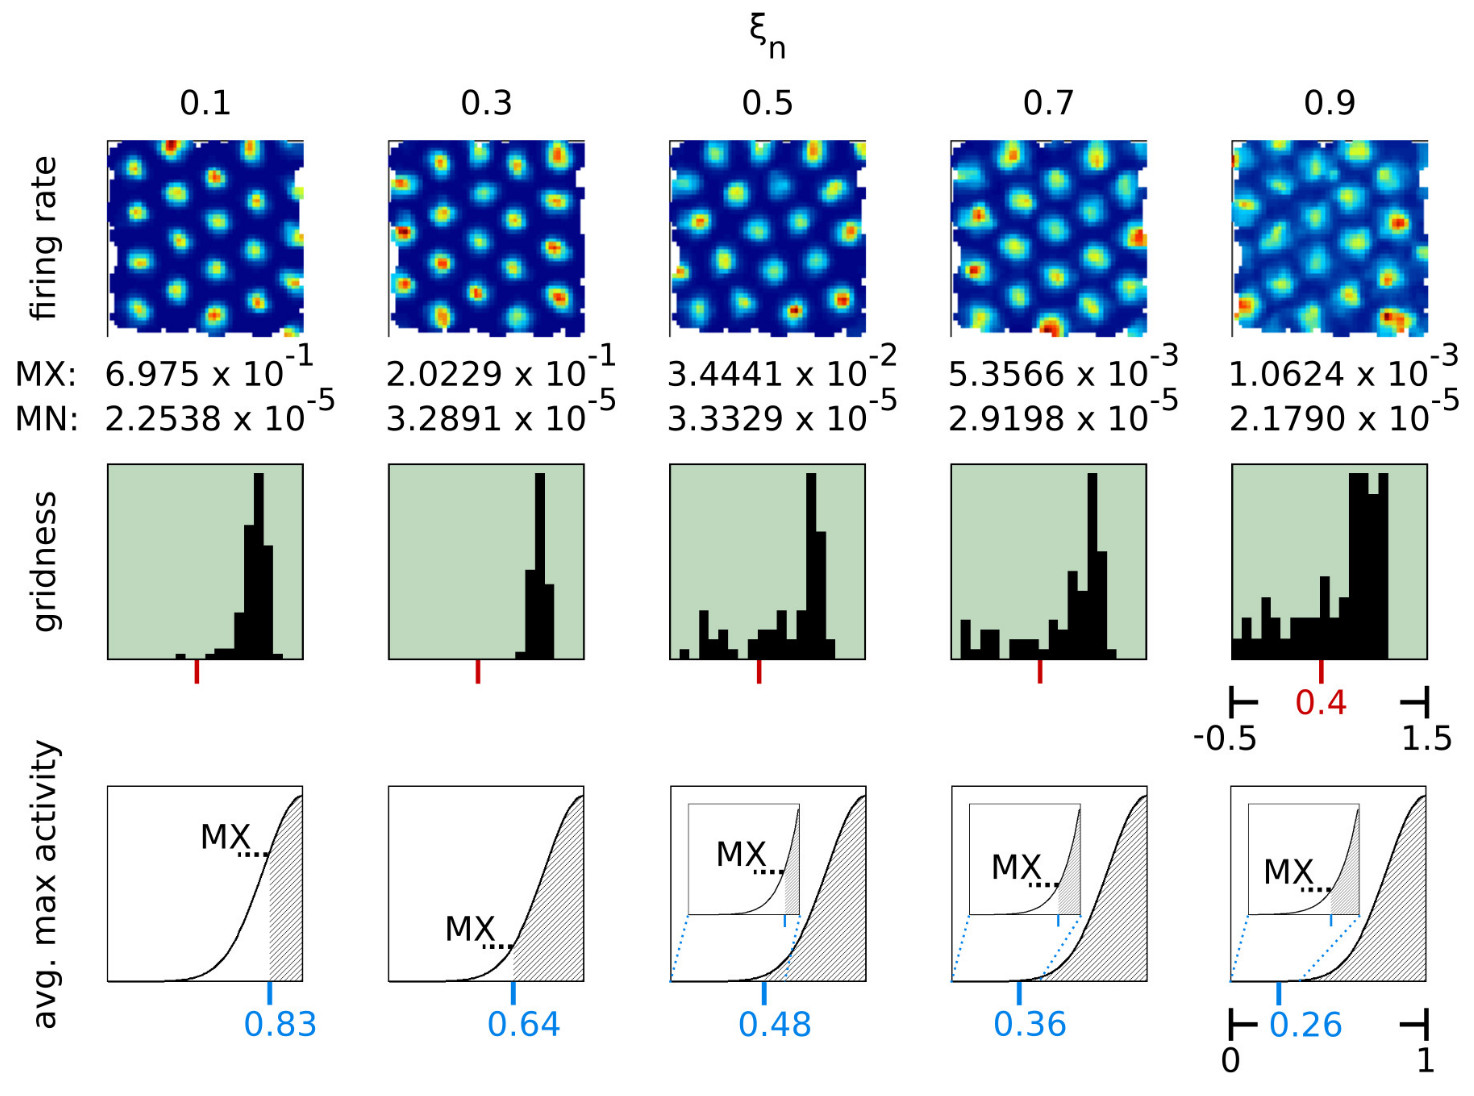
\includegraphics[width=\linewidth]{diss/noisecomp.jpg}

\vspace{-0.5em}
\caption{\justifying\scriptsize Artificial rate maps (top), gridness distributions 
(middle), and activity function plots (bottom) of simulation runs with varying 
levels \(\xi\) of noise (columns) added to the inputs. Details 
in~\cite{Kerdels2019a}.}
\end{figure}
}{0.5}{

\justifying
We investigated the noise resilience of our computational grid cell model and 
were able to demonstrate that our {\bf model is very robust to noise} due to the
prototype-based nature of the underlying algorithm\cite{Kerdels2016c}.

\vspace{2.25em}
In a follow-up work we present a {\bf noise compensation mechanism} that aims at 
equalizing the level of output activity across changing levels of 
noise\cite{Kerdels2019a}.

}

\vspace{-1em}

\begin{center}
\rule{2cm}{0.4pt}\\[0.5em]
\end{center}

\fc{Kerdels2016c}{publications/2016-04/2016-04}\nombestpaper\\[1em]
\fc{Kerdels2019a}{publications/2019-01/2019-01}

\end{frame}


\begin{frame}{Grid Cell Modeling \sof{5}{5}}

\vspace{1.5em}
\justifying
The dentate gyrus (DG) in the hippocampus of the mammalian brain is known to 
exhibit strong {\bf pattern separation}. However, how this pattern separation 
arises in the DG is not well understood.

\vspace{1em}
Based on our grid cell model we offer a novel hypothesis regarding this 
question by demonstrating that {\bf pattern separation can already be performed 
by entorhinal grid cells}, which are located just one synapse upstream of the 
DG~\cite{kerdels2017}.

\begin{columns}[t]
\begin{column}{0.2\textwidth}
\begin{figure}
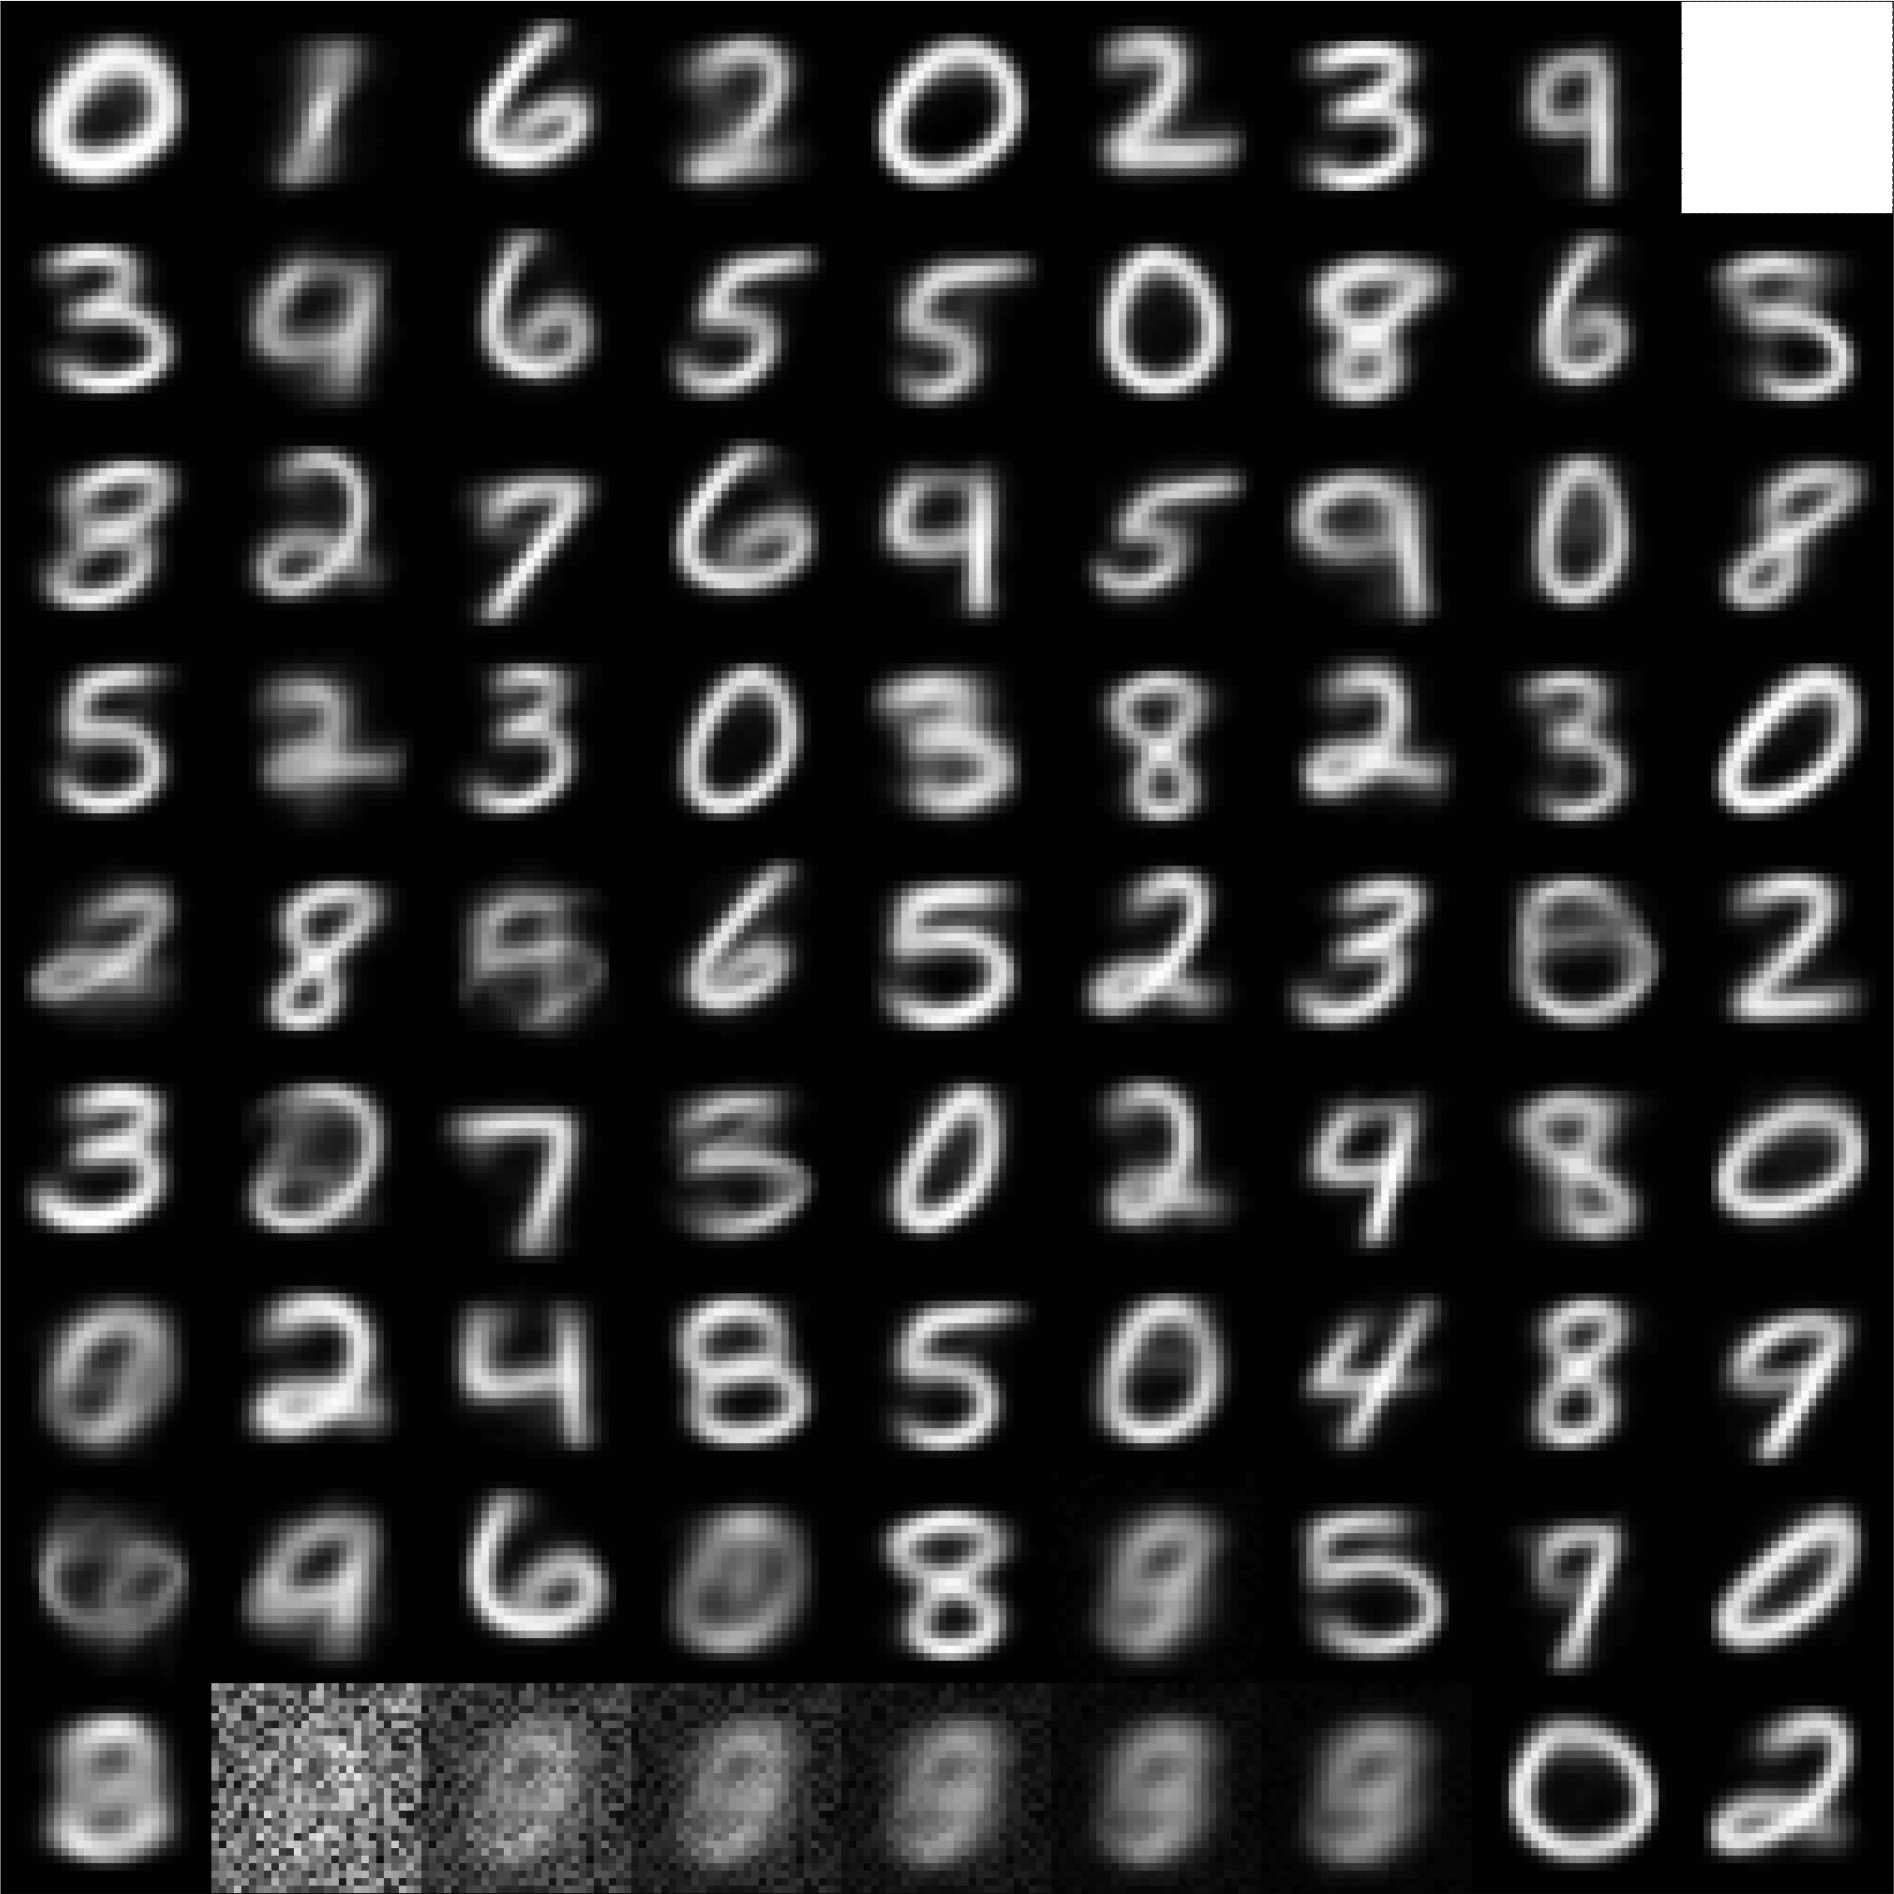
\includegraphics[width=\linewidth]{diss/80_p20.jpg}

\vspace{0.6em}
\caption{\justifying\scriptsize Examples of 80 prototypes that form the input space 
representation of a simulated grid cells~\cite{kerdels2017}.}
\end{figure}
\end{column}
\begin{column}{0.35\textwidth}
\begin{figure}
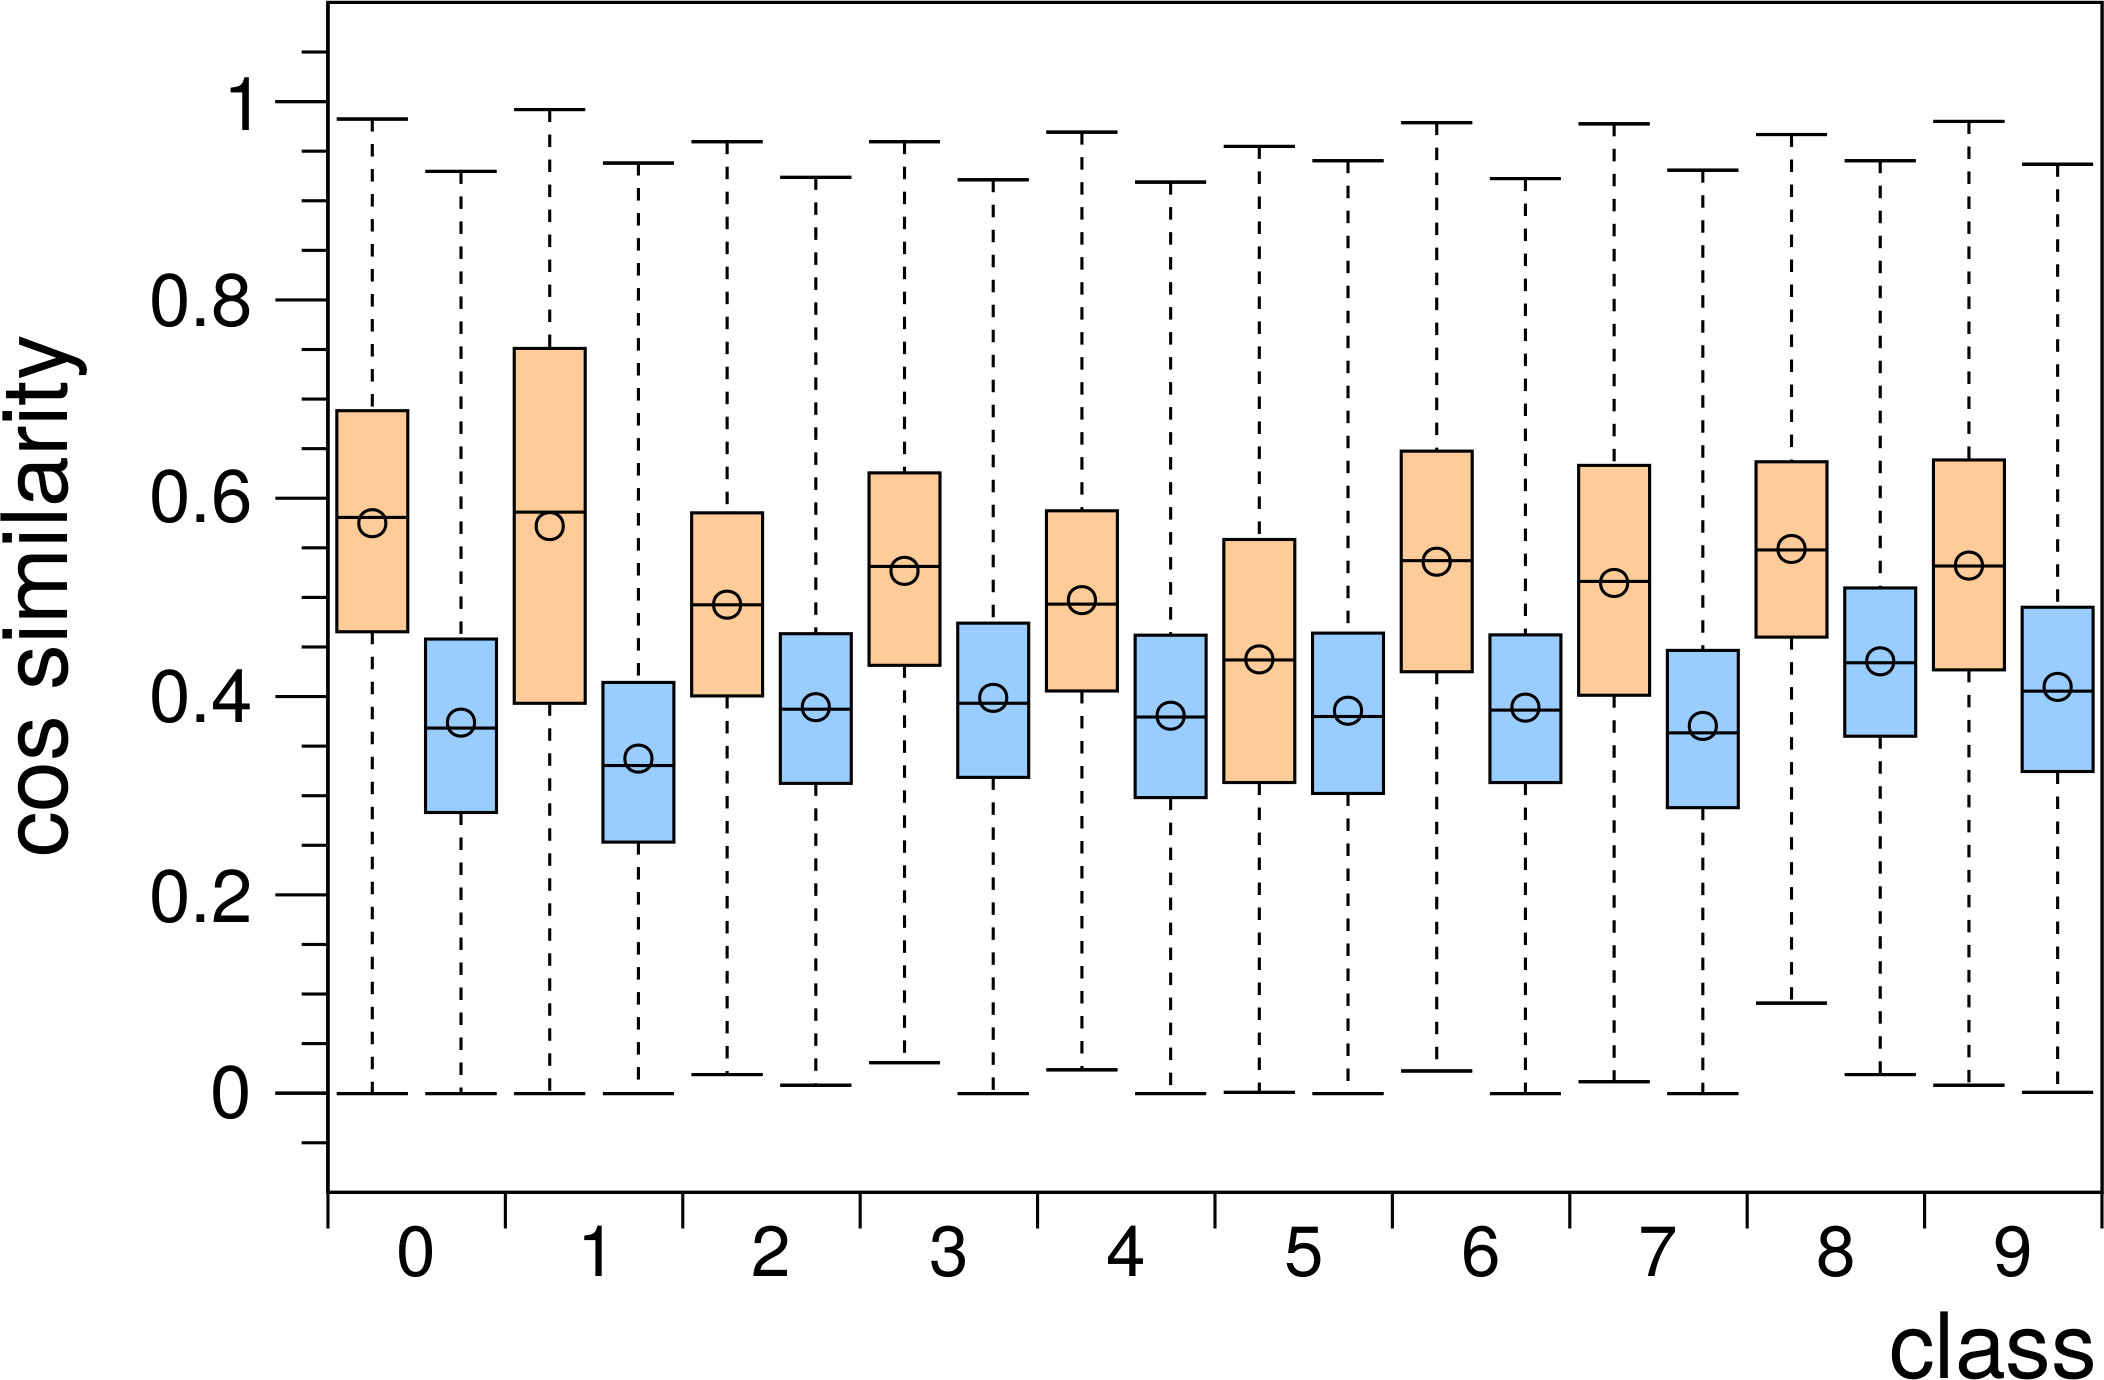
\includegraphics[width=\linewidth]{diss/MNIST_dist.jpg}

\vspace{-0.5em}
\caption{\justifying\scriptsize Box plot of the intra-class (orange, left 
columns) and inter-class (blue, right columns) cosine similarity distributions 
occurring in the MNIST dataset. Details in~\cite{kerdels2017}.}
\end{figure}
\end{column}
\begin{column}{0.35\textwidth}
\begin{figure}
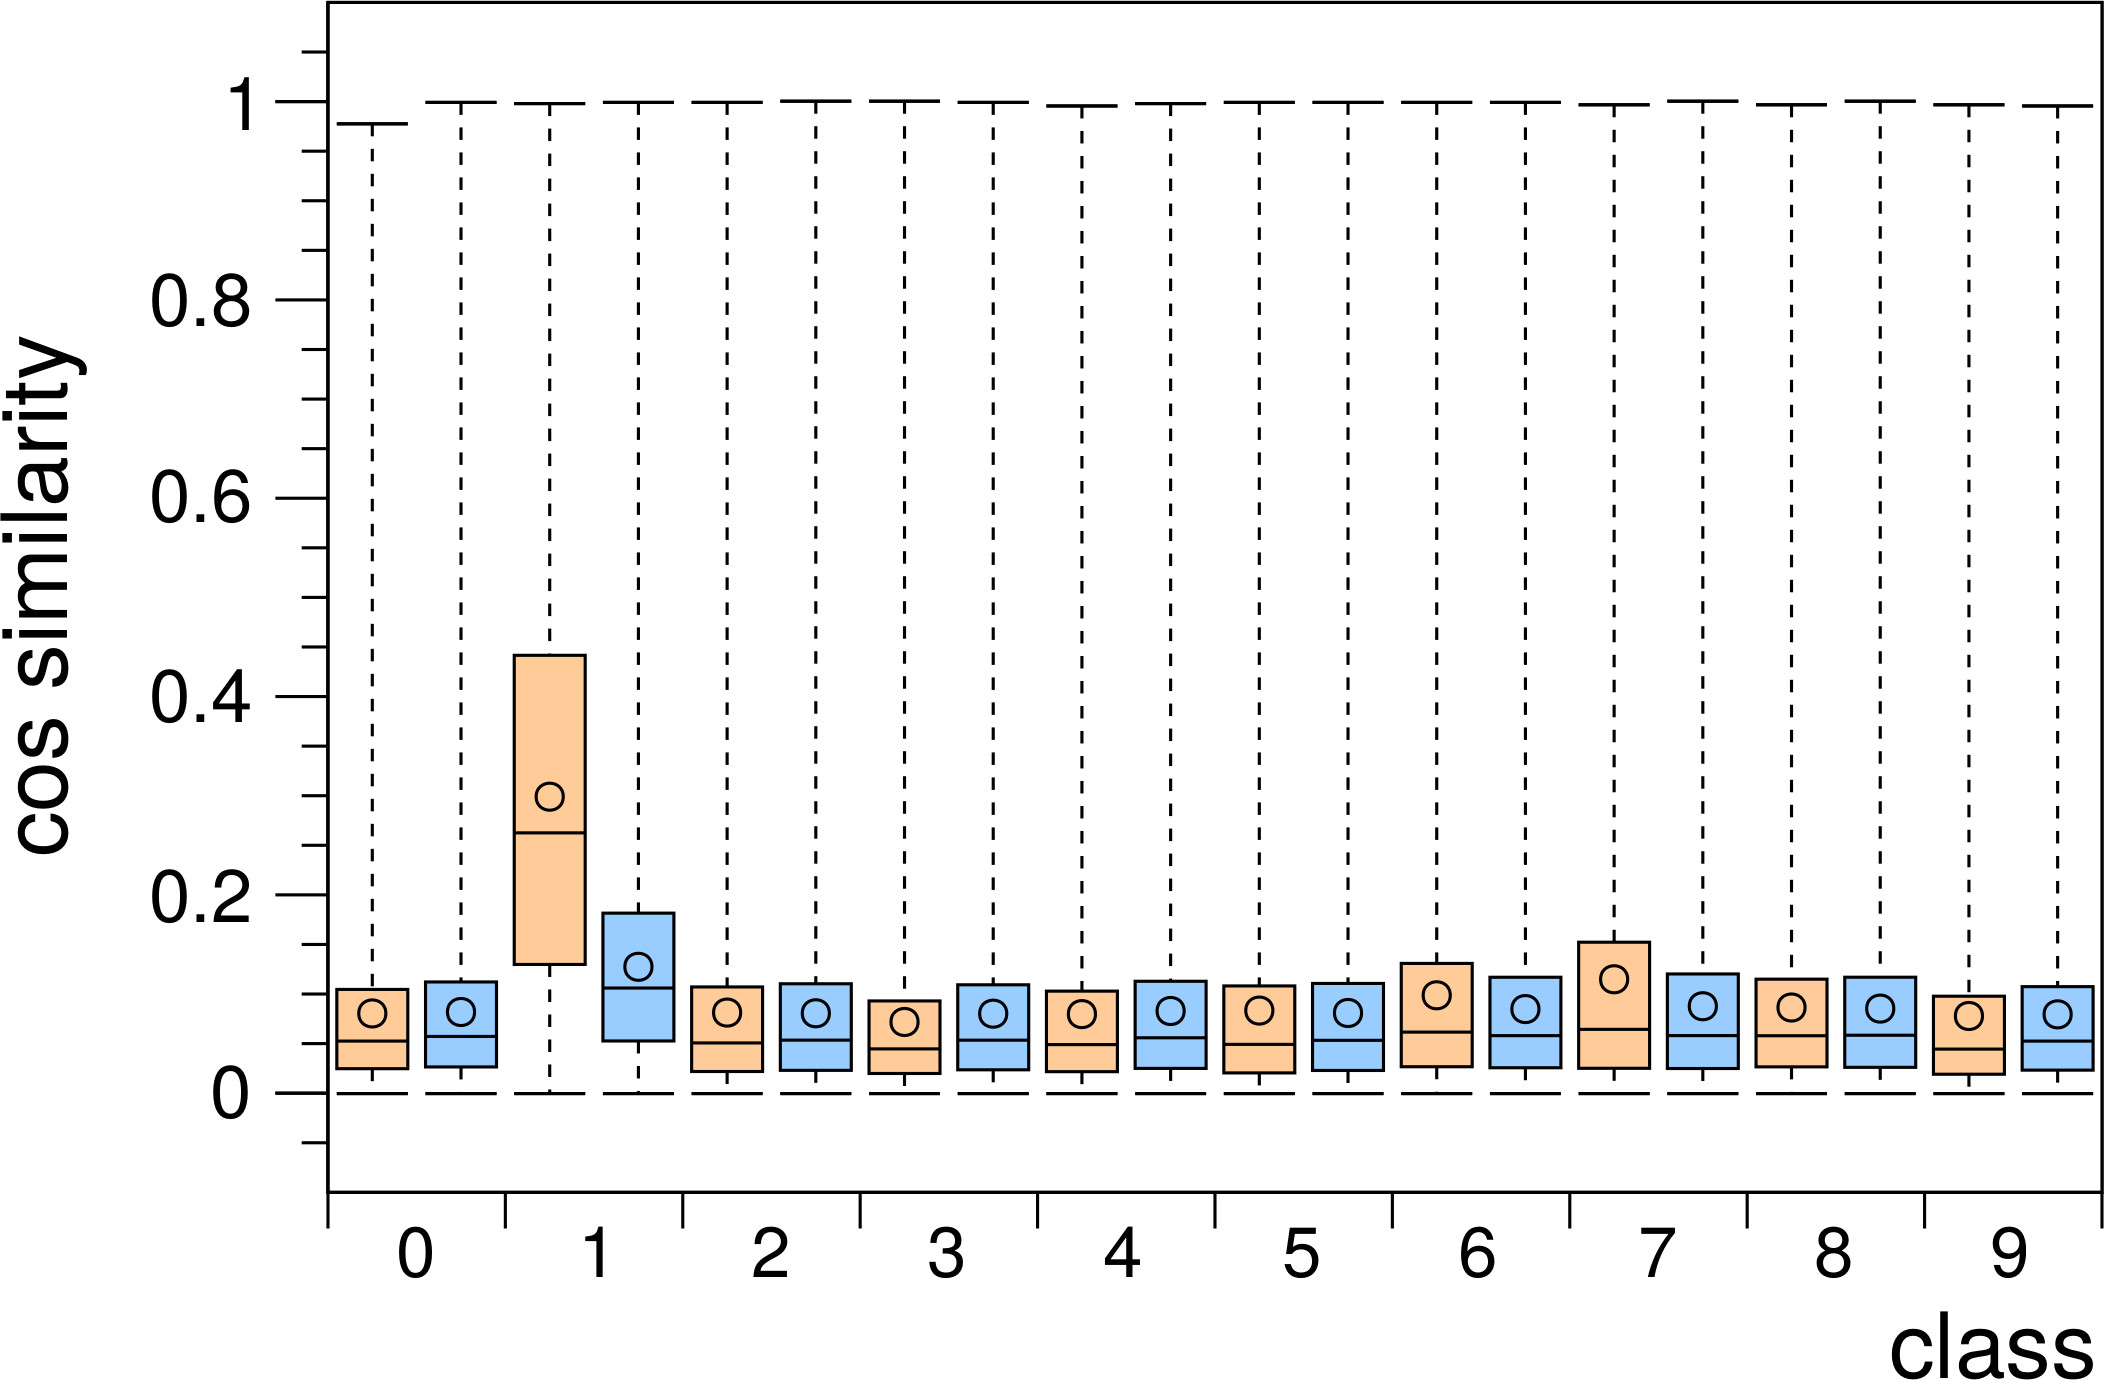
\includegraphics[width=\linewidth]{diss/all_80.jpg}

\vspace{-0.5em}
\caption{\justifying\scriptsize Box plots the intra- and inter-class cosine 
similarity distributions occurring in simulated multimodal activity vectors of 
grid cell groups encoding the top, bottom, left, or right halves of the MNIST 
input samples. Details in~\cite{kerdels2017}.}
\end{figure}
\end{column}
\end{columns}	

\vspace{-0.5em}

\begin{center}
\rule{2cm}{0.4pt}\\[0.5em]
\end{center}

\fc{kerdels2017}{publications/2017-01/2017-01}

\end{frame}

